% Added by BB
%% This holds definitions of macros to enforce consistency in names.

% This file is the sole location for such definitions.  Check here to
% learn what there is and add new ones only here.  

% also see units.tex for units.  Units can be used here.

%%% Common terms

% Check here first, don't reinvent existing ones, add any novel ones.
% Use \xspace.

%%%%% Anne adding macros for referencing CDR volumes and annexes Apr 20, 2015 %%%%%
\def\expshort{DUNE\xspace}
\def\explong{The Deep Underground Neutrino Experiment\xspace}

\def\volintro{CDR Volume 1: Introduction\xspace}
\def\volphys{CDR Volume 2: Physics with DUNE at LBNF\xspace}
\def\vollbnf{CDR Volume 3: LBNF\xspace}
\def\voldune{CDR Volume 4: The DUNE Detectors\xspace}

\def\anxcernproto{Annex: CERN Single-phase Prototype Detector Proposal\xspace}
\def\anxlbnefd{Annex: LBNE FD Design Jan 2015\xspace}
\def\anxrates{Annex: Data Rates\xspace}
\def\anxndref{Annex: Near Detector Reference Design\xspace}
\def\anxlbnoa{Annex: LAGUNA/LBNO Part 1\xspace}
\def\anxlbnob{Annex: LAGUNA/LBNO Part 2\xspace}
\def\anxlbnesci{Annex: LBNE: Exploring Fundamental Symmetries of the Universe\xspace}
\def\anxdualrpt{Annex: Progress report on LBNO-DEMO/WA105 (2015)\xspace}
\def\anxdualtdr{Annex: WA105 TDR\xspace}

\def\cernsingleproto{Name of CERN Single-Phase Prototype\xspace}
\def\cerndualproto{Name of CERN Dual-Phase Prototype\xspace}

% Things about oscillation
%
% example: \dm{12}
\newcommand{\dm}[1]{$\delta m^2_{#1}$\xspace}
% example \sinstt{12}
\newcommand{\sinstt}[1]{$\sin^22\theta_{#1}$\xspace}
% example \deltacp
\newcommand{\deltacp}{$\delta_{\rm CP}$\xspace}
% example \nuxtonux{\mu}{e}
\newcommand{\nuxtonux}[2]{$\nu_{#1} \to \nu_{#2}$\xspace}
\newcommand{\numutonumu}{\nuxtonux{\mu}{\mu}}
\newcommand{\numutonue}{\nuxtonux{\mu}{e}}
\newcommand{\numu}{$\nu_\mu$\xspace}
\newcommand{\nue}{$\nu_e$\xspace}
\newcommand{\anumu}{$\bar\nu_\mu$\xspace}
\newcommand{\anue}{$\bar\nu_e$\xspace}

% Names
\newcommand{\cherenkov}{Cherenkov\xspace}
\newcommand{\kamland}{KamLAND\xspace}
\newcommand{\kamiokande}{Kamiokande\xspace}
\newcommand{\superk}{Super--Kamiokande\xspace}
\newcommand{\miniboone}{MiniBooNE\xspace}
\newcommand{\minerva}{MINER$\nu$A\xspace}
\newcommand{\nova}{NO$\nu$A\xspace}
\newcommand{\SURF}{Sanford Underground Research Facility\xspace}

\def\Ar39{$^{39}$Ar}
\def\driftvelocity{\SI{1.6}{\milli\meter/\micro\second}\xspace}

%\begin{document}
% PLEASE FOLLOW POSTED GUIDELINES!!

% Please see the two LAr CDR 'guidelines' writeboards in basecamp
% at https://lbne-doc.basecamphq.com/projects/4264323/writeboards
% One is for text, the other for images and figures 

\def\NOvA{NO$\nu$A }
\chapter{Veto System}
\label{ch:veto}

% I have to figure out why the captions are so far below the diagrams themselves. Waiting for serial num for my adobe photoshop app... 7/23 AH

The scope of the WBS 130.5.7 Liquid Argon Detector Veto subsystem includes the design, procurement, fabrication, testing, delivery and installation oversight of 18,300 liquid scintillator veto counters embedded in the cavern walls and 558 \NOvA modules across the top of the LAr detector that meet the required performance for cosmic-ray event identification in the LBNE liquid argon (LAr) detector.  This chapter describes a reference design for the Veto subsystem adapted from the NO$\nu$A  detector.

\section{Background-Rejection Requirements for Physics}

\subsection{Accelerator Neutrinos}

The rate of cosmic-ray muons in the detector at the 800L is 0.06~Hz/m$^2$ or $\sim$ 1~Hz/APA cell. During a drift time of 2.3 ms, 0.002 cosmic rays will pass through the active volume of one APA cell, resulting in a timing rejection factor of $\sim$400. Since accelerator neutrino signal events must point back to Fermilab and be time correlated with the beam spill, the high granularity of the detector will allow identification and removal of the cosmic muons from the data, introducing only a small ($< 0.1$\%) inefficiency to the active detector volume.  Most of the accelerator-induced events will remain unobscured.  In short, a cosmic ray veto is not required to study neutrino interactions at the 800L.

\subsection{Nucleon Decay}

The depth requirement for proton-decay experiments is dominated by the livetime loss due to event overlap with cosmic muons in both time and space.  A liquid argon detector will have much less deadtime loss at shallow depths than a water Cherenkov detector since the fine segmentation in space and drift time allow either trigger-based or offline-analysis exclusion of smaller volumes of the detector around each passing muon. With mountainous overburden of only 200~m and a veto counter, Reference \cite{bueno-pdk} estimates an effective loss of detector mass of less than 4\% for a 100-kton liquid argon detector (GLACIER). 

The most serious source of nucleon-decay background for the SUSY-favored $p \rightarrow \nu K^+$ decay mode are $K^0_L$ mesons produced by spallation of cosmic-ray muons in the rock surrounding the detector. The effective interaction length of these $K^0$'s in liquid argon is 86~cm. These neutral kaons may enter the detector and produce a $K^+$ via charge-exchange which mimics the nucleon decay signal.  The cosmic muons that pass through the rock near the cavern wall at small zenith angle as shown in figure \ref{fig:spallation} produce the largest contribution to the $K^0$ background. Muons traveling at a larger zenith angle are unlikely to produce a forward-going $K^0$ that is unaccompanied by the interacted muon.

\begin{figure}[h]
\centering
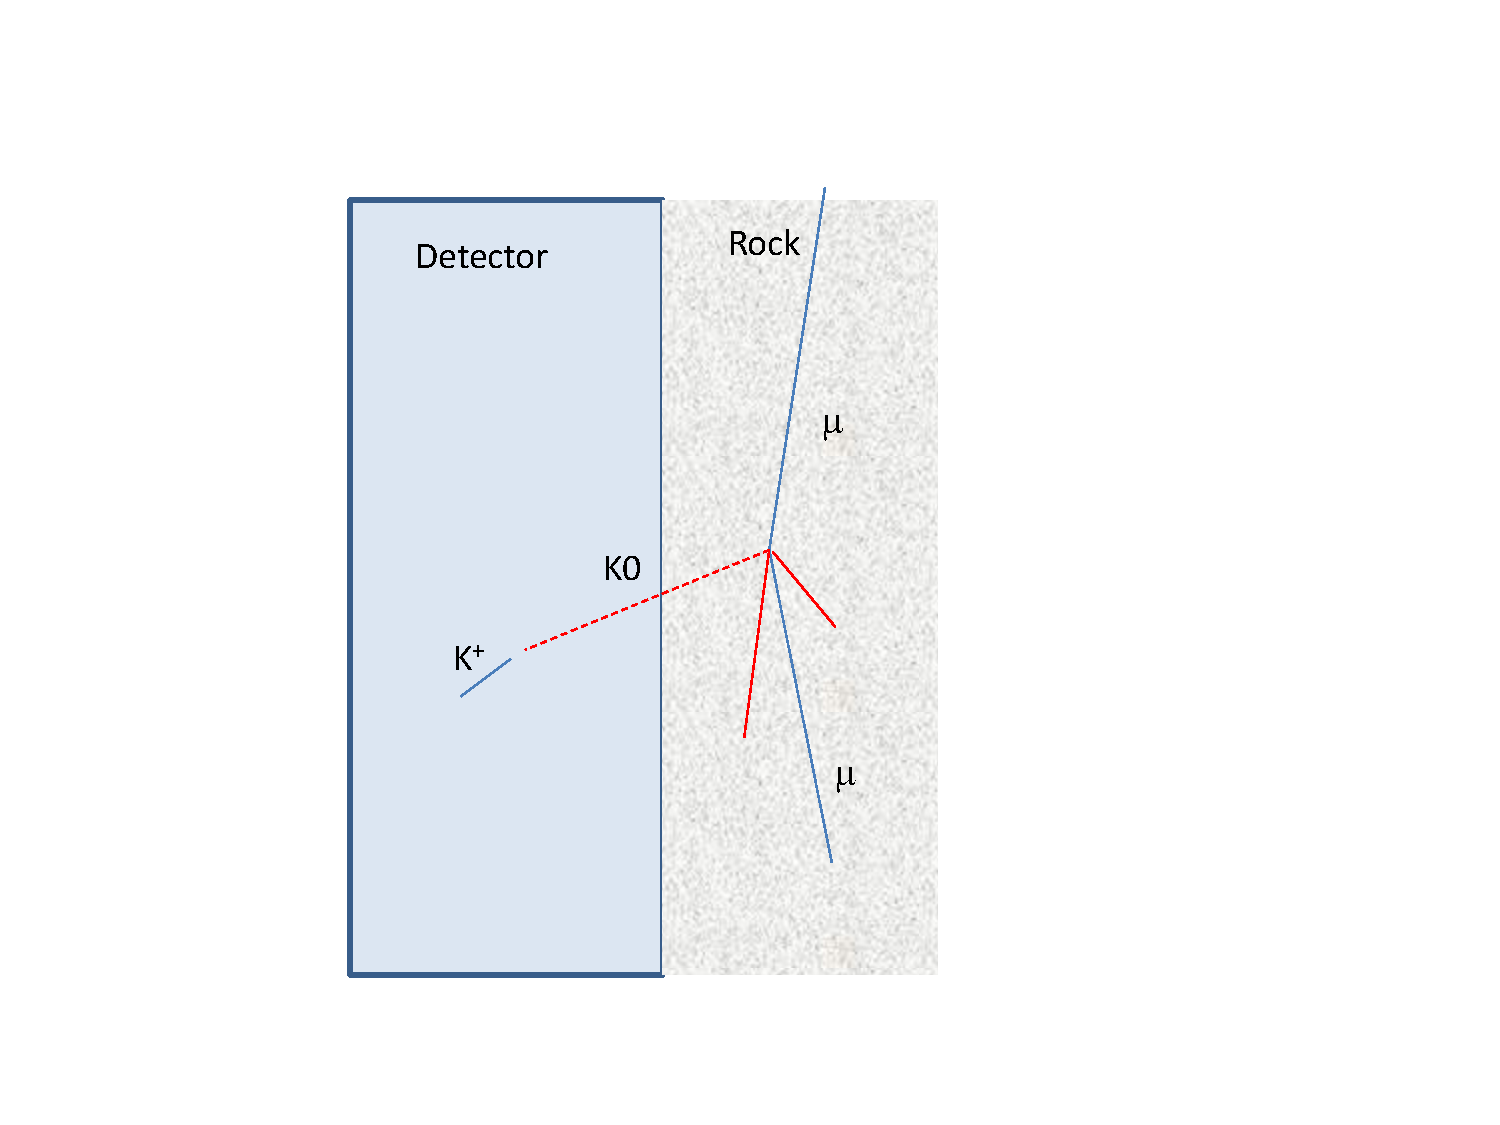
\includegraphics[width=\textwidth]{chapter-07_spallation.pdf}
\caption{Cosmic-ray spallation background to proton decay in the p $\rightarrow$ $\nu K^+$.}
\label{fig:spallation}
\end{figure}

The veto described in the following section is designed to reduce the background in the $p \rightarrow \nu K^+$ mode to a negligible level based on these arguments. Monte Carlo simulation of the proposed veto system is clearly required.

\section{Veto System Description}

\begin{figure}[h]
\centering
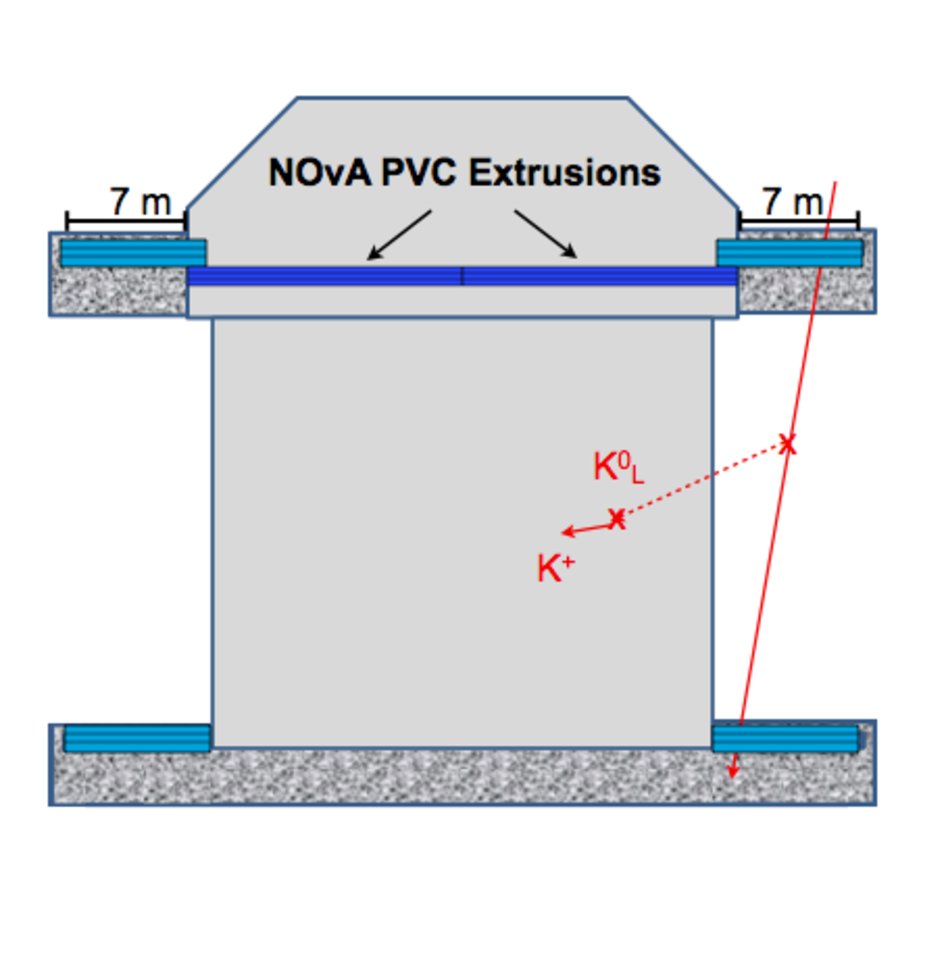
\includegraphics[width=.7\textwidth]{v5ch07-vetoend}
\caption{End view of the cavern wall showing veto tubes embedded in concrete in the walls of the cavern.}
\label{fig:vetoend}
\end{figure}

The aforementioned GLACIER detector concept is an upright cylindrical tank of 20~m height and 70~m diameter, surrounded by annular veto detectors that extend 3~m into the surrounding rock. An additional 3 -- 5-meter fiducial cut was made inside the detector to reduce the spallation background in the  $\nu K^+$ channel to 0.1 event per year. In contrast, we propose to extend the veto counters 7~m into the rock to obviate the need for a fiducial cut. The interaction length of rock is roughly half the interaction length of liquid argon, so each meter of rock should provide twice the neutral-kaon attenuation as each meter of liquid argon. 

The 800L LAr40 veto system is shown in figures \ref{fig:vetoend} and \ref{fig:vetotube}.  The cavern will be 
constructed with 9150 9m long 4" square steel tubes in the cavern walls (with $\sim2$ meters sticking out) at the top of the cavern, and a similar number of 9m long 4" square steel tubes in the cavern walls at the bottom.  Square PVC tubes will be inserted into the steel tubes, and filled with liquid scintillator and wavelength shifting fiber (WLS), similar to the method used by \NOvA.  Coverage across the top of the detector is provided by 3 layers of 2 columns of 12m long \NOvA PVC modules laid across the truss at the top of the detector (Fig.~\ref{fig:vetoOnTruss}).   Both ends of the WLS fiber are attached to a single-channel Avalanche Photo-Diode (APD) mounted on the same end of the cell through which scintillator is filled. 

The design and the cost estimate are adapted from the \NOvA detector.  Both the cavern and steel tubes are provided by WBS 1.6.  The veto system provides the PVC inserts, \NOvA PVC modules, WLS, scintillator and Avalanche Photo-Diodes (APDs) and associated electronics for readout.  

\begin{figure}[h]
\centering
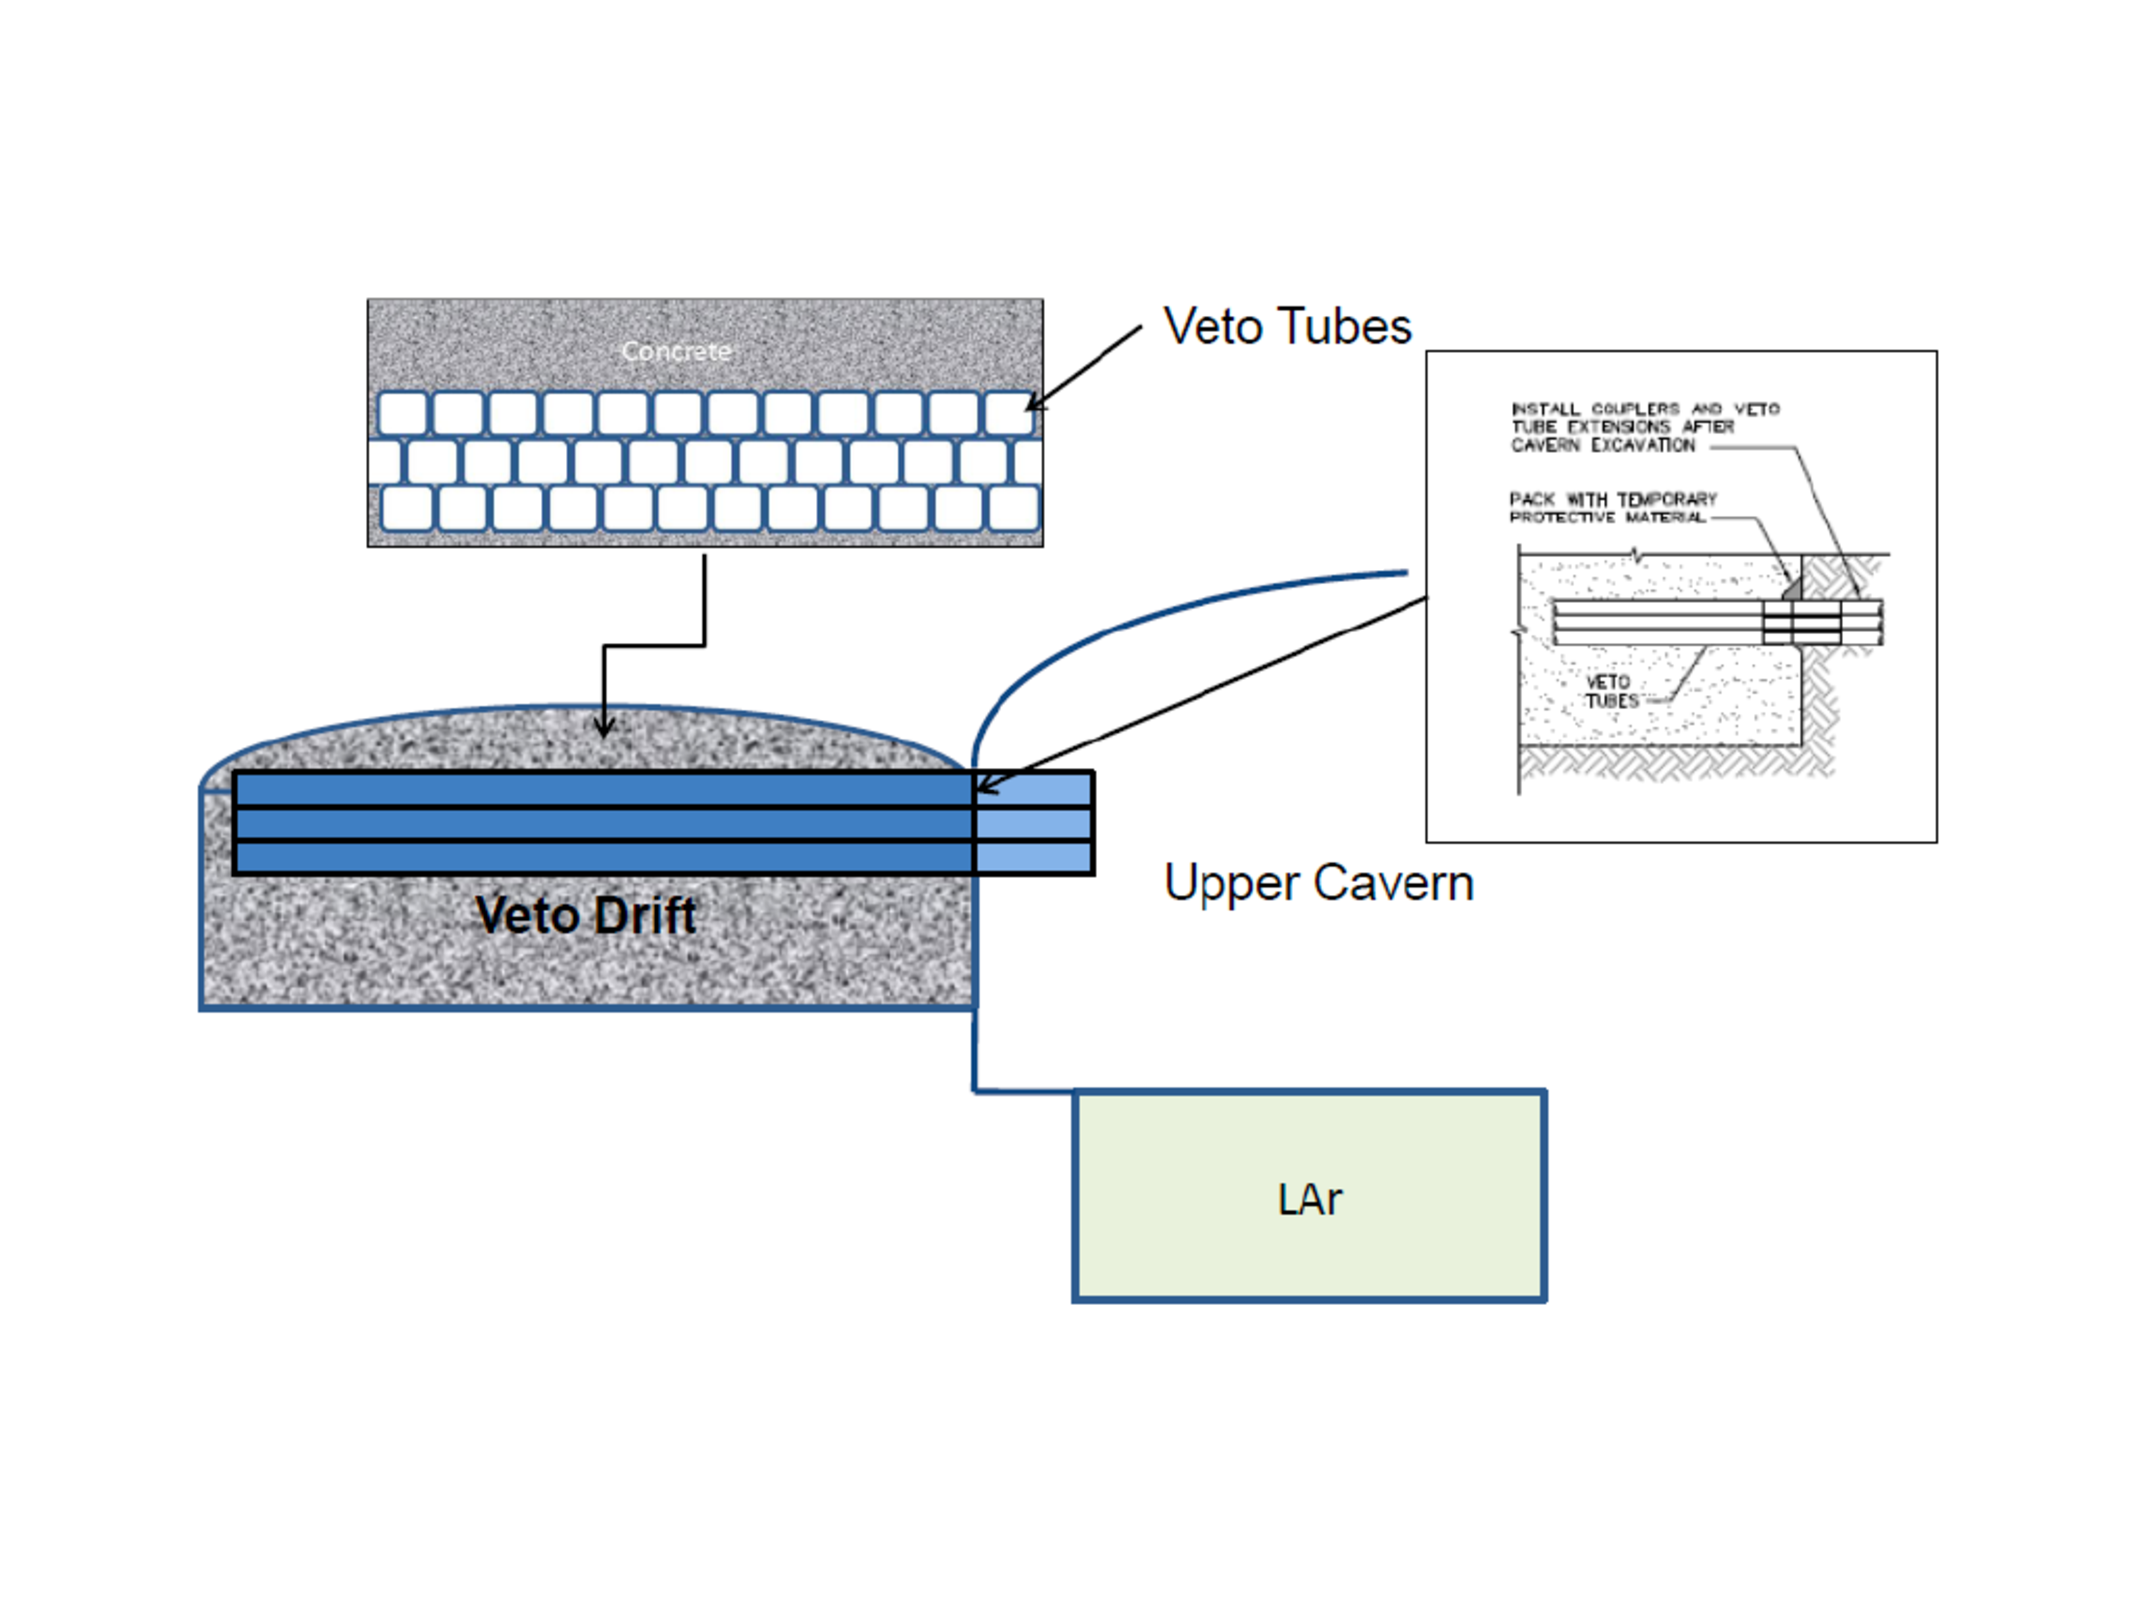
\includegraphics[width=.9\textwidth]{v5ch07-vetotube}
\caption{Conceptual layout of the veto tubes.}
\label{fig:vetotube}
\end{figure}

\begin{figure}[h]
\centering
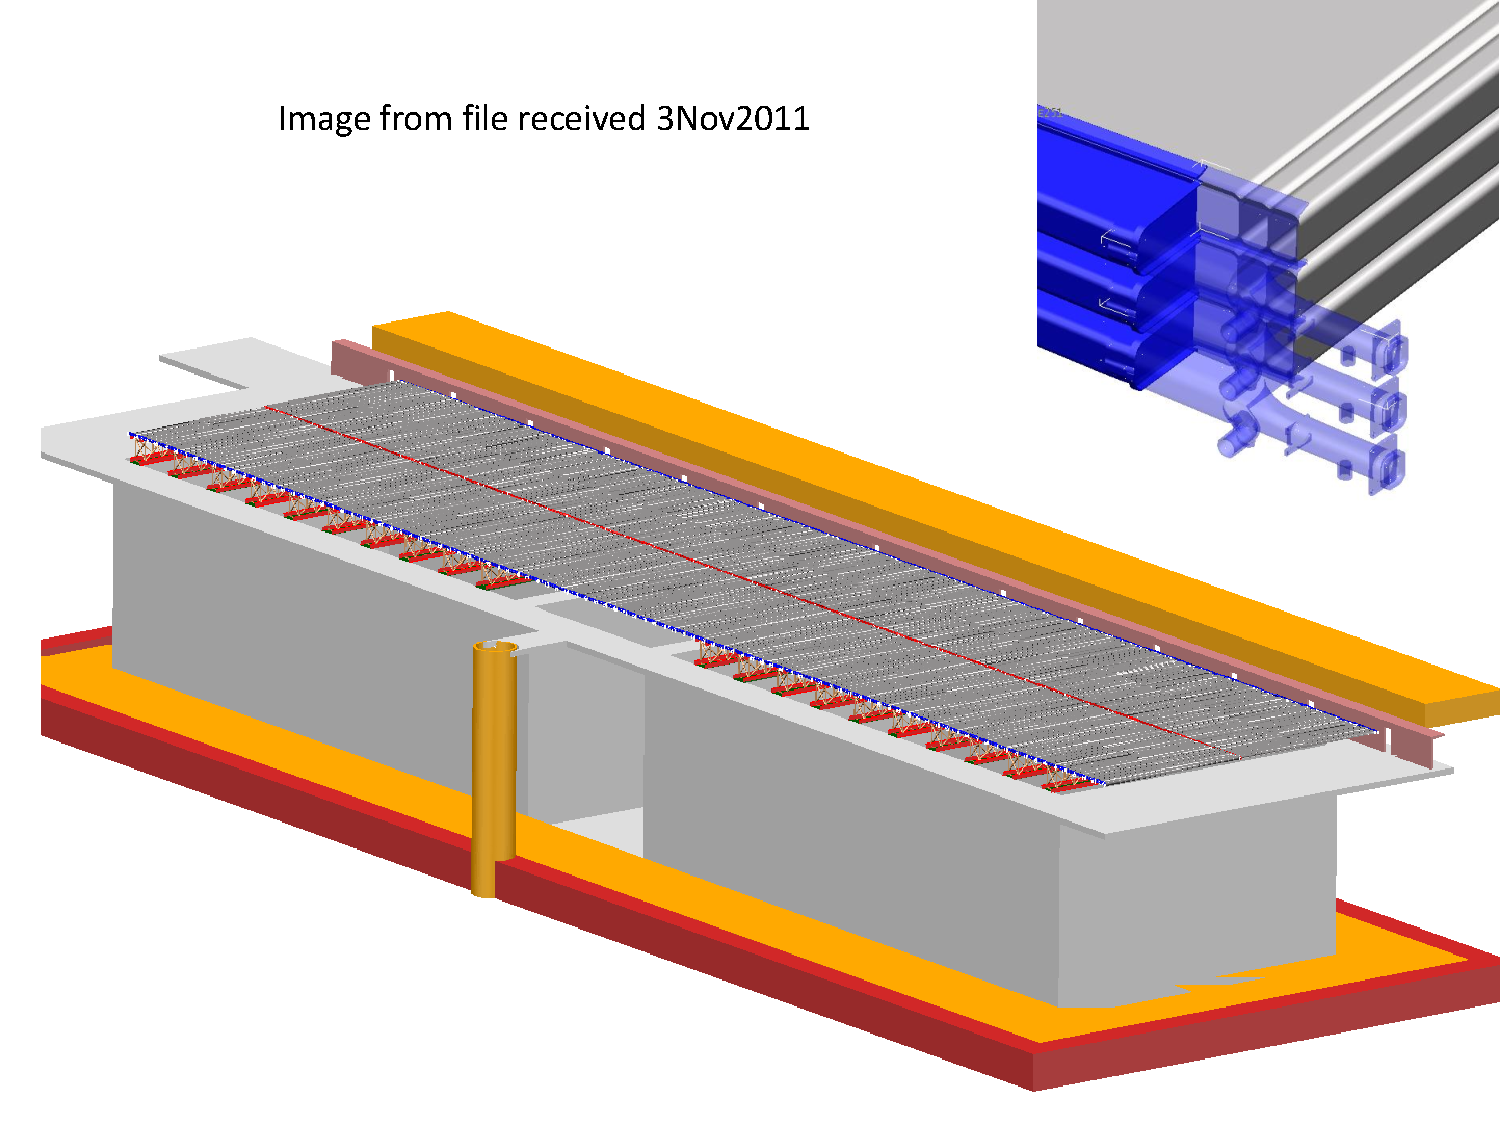
\includegraphics[width=.75\textwidth]{v5ch07-vetoOnTruss}
\caption{Conceptual layout of \NOvA-like modules across the 800L cavern truss.}
\label{fig:vetoOnTruss}
\end{figure}

Each \NOvA module consists of 32 detector cells built from two separate 16 cell extrusions epoxied together. The \NOvA detector cell is 3.7~cm $\times$ 5.9~cm $\times$ 15.3~m. Each cell contains liquid scintillator and a looped WLS fiber that is routed to a single channel of an Avalanche PhotoDiode (APD) array. Cosmic ray tests, summarized in figure \ref{fig:nova_pe}, have shown that $\sim$35 photo-electrons are observed at the APD from a vertical minimum-ionizing particle passing through the far end of the 15.3-m-long cell. The RMS width of the cosmic-ray signal is 11 photo-electrons, or 31\%. To reduce the amount of noise read out from the detector to one-third of the expected cosmic muon rate at the far detector, \NOvA has set a threshold of 15 photo-electrons which corresponds to a noise-hit probability of $10^{-4}$.  This results in an inefficiency at the percent level for minimizing-ionizing particles passing through the far end of the detector.

\begin{figure}[h]
\centering
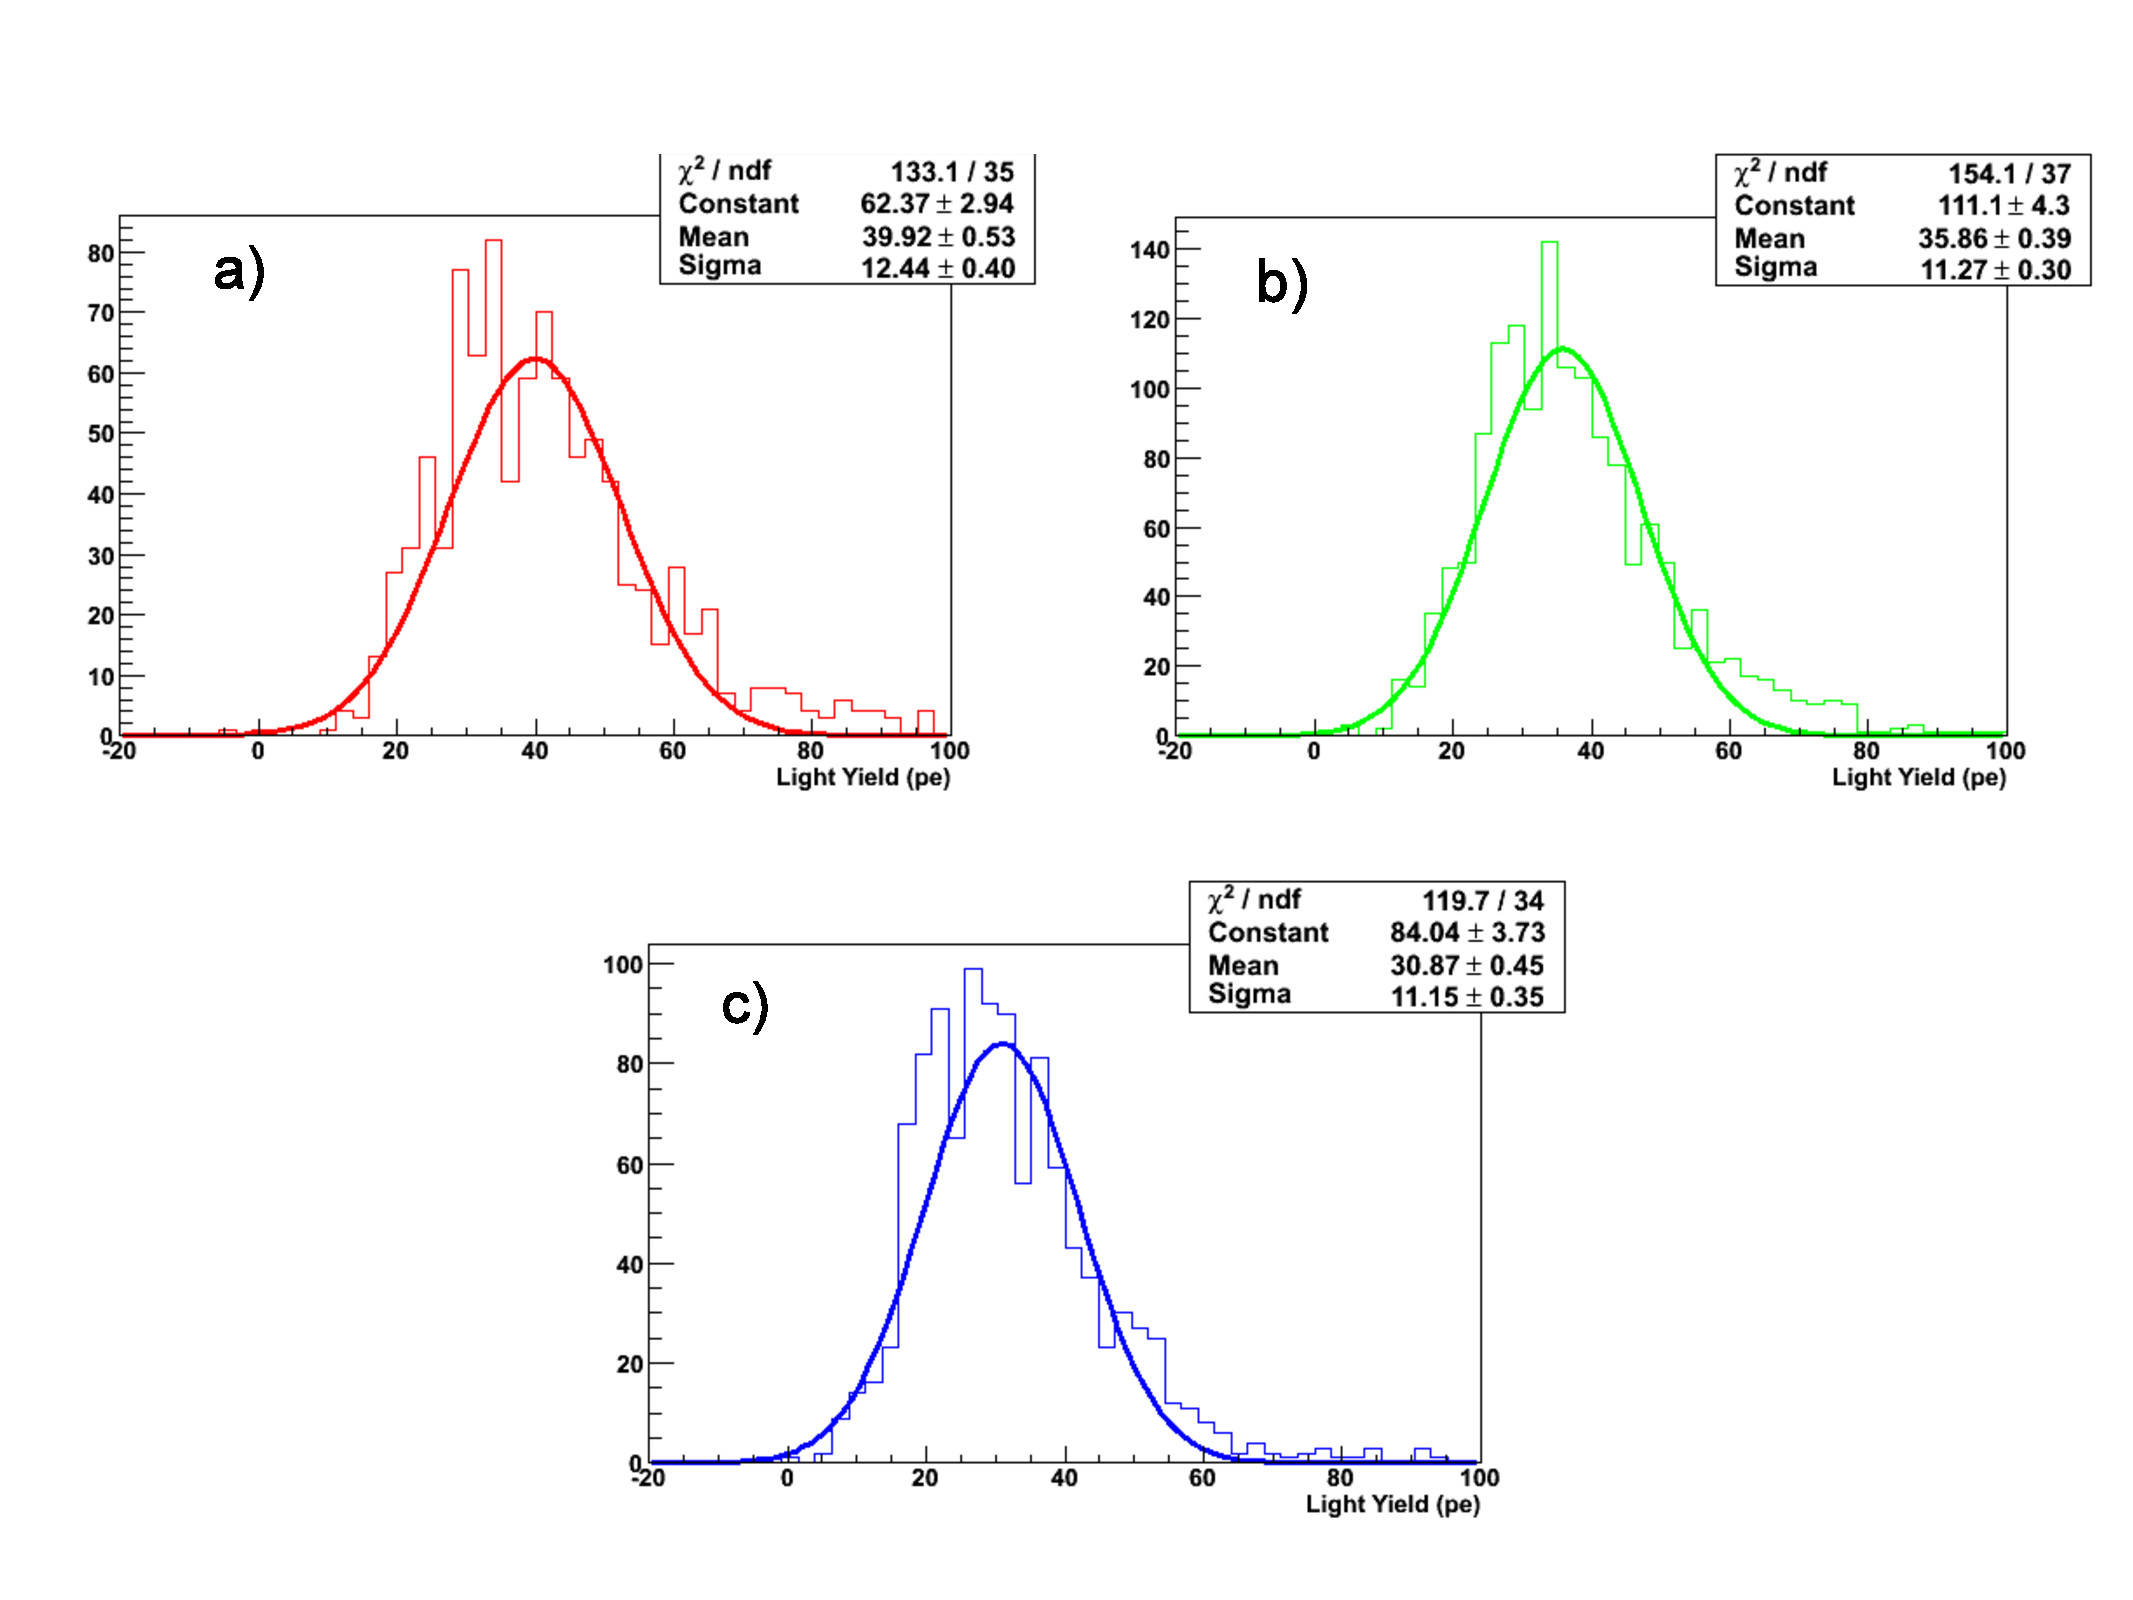
\includegraphics[width=.7\textwidth]{chapter-07_vetope}
\caption{Distributions of light yield measurements on three different \NOvA test cells using cosmic ray muons. \cite{novatdr} }
\label{fig:nova_pe}
\end{figure}

We estimate the performance of the proposed cavern-wall veto tube design by scaling the number of photo-electrons expected in at the far end of a \NOvA cell to the far end of the proposed veto cell.  The attenuation of scintillator light in a \NOvA cell has been measured parameterized as a double exponential \cite{NOvA-docdb3290}:
\begin{eqnarray*}
N(\mathrm{pe}) & = & N_0( 0.31(\exp(-x/2.9) + \exp(-(2L-x)/2.9)) + \\
& & 0.17(\exp(-x/8.5)+\exp(-(2L-x)/8.5)))
\end{eqnarray*}
where $x$ is the distance to the readout-end and $L$ is the length of the module.  For $x=L=15.3$m, $N$(pe)=35.  Using this same attenuation (which is dominated by attenuation in the wavelength-shifting fiber), one gets 86 pe for a mip passing through the end of a 9-m long NOvA cell.  Scaling again by the ratio of the cell dimensions for the two cell configurations (7.8~cm/3.7~cm $\simeq$ 2.1), we therefore expect $\sim 180$ pe for a mip passing through the end of a 9-m long cavern wall cell.  54 pe are expected for a mip passing through the end of a 12-m long \NOvA module at the top of the detector.  Ample light is produced such that the threshold could be set to the 15 photo-electron threshold used by \NOvA without introducing a significant detection inefficiency.

Three rows of veto counters are arranged in a staggered pattern to maximize the angular coverage. This configuration does not provide any stereo angle information to determine the distance from the cavern wall to the cosmic ray. Pulse-height information can conceivably be used for this purpose, however this information is not required for the purpose of the veto.

The veto will be implemented in the data acquisition as an additional detector system. The veto detectors will be sampled by ADCs operating at 2~MHz and merged with the TPC data stream. The veto system will be used to reject a reconstructed $K^+$ as a proton-decay candidate if a nearby veto counter has a pulse height consistent with a minimum-ionizing particle.

